\subsection[Agent Roles and Actions]{Agents Roles and Actions$^{\star,\circ}$}\label{fun:mapc_roles}
% This is the text from the TOC:
% What is the general scenario? Agents on mars trying to find water in a competitive manner against another team. Explain the concept of zones, gaining points, achievements and also how agents differ from each other.
% I've put this section first so the later chapters can already rely on the reader knowing what the scenario is about. Furthermore, we can then directly rule out concepts which we are presenting by applying them theoretically onto the scenario/our needs.
\todo{Write this section}
This section presents the basic behaviour of our agents given the actions that all agents share.
Every agent team in the MAPC Scenario consists of 28 agents.
These agents are divided into five roles: the Explorer agent, the Repairer agent, the Saboteur agent, the Sentinel Agent and the Inspector agent.
\begin{figure}[ht]
  \centering
  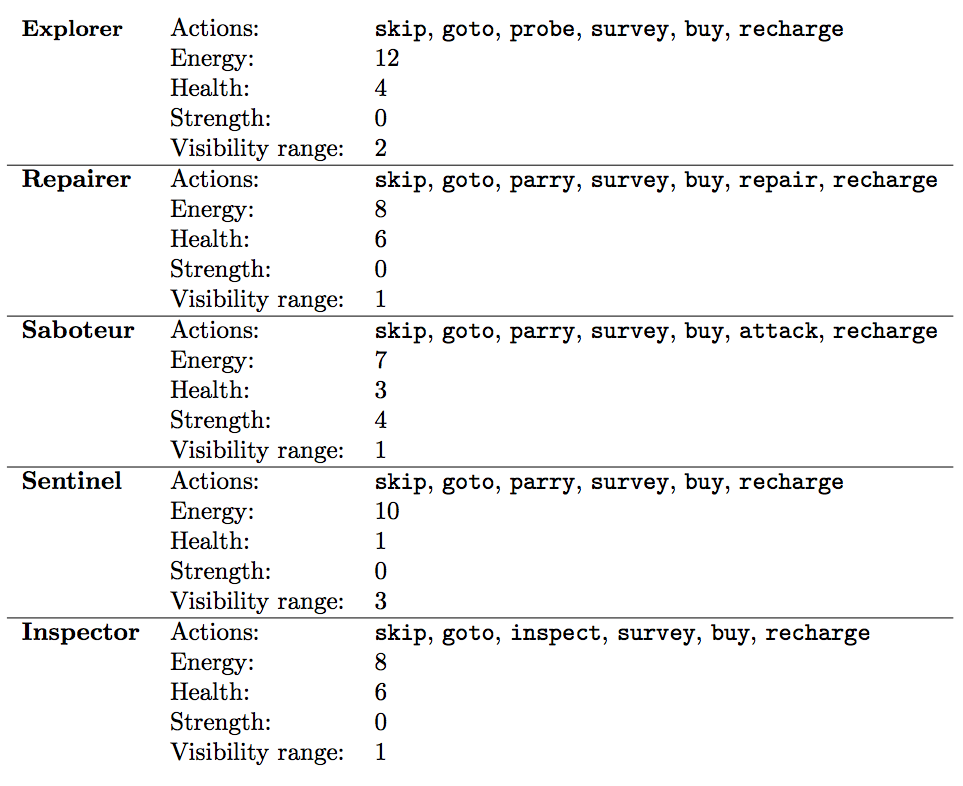
\includegraphics[width=0.9\linewidth]{images/roles.png}
  \caption{The different agent roles in the MAPC scenario \cite{ahlbrecht_mapc_2014}.}
  \label{fig:fun:roles}
\end{figure}
As shown in \autoref{fig:fun:roles}, each role is given different values in their attributes of maximum energy, health or visibility range.
Moreover, the saboteur agent has a strength value, because it is the only agent which can attack enemy agents.
There are six agents of each role except the Explorer agent role of which there are four agents.
Except for the Sentinel role, all other roles allow their correpsonding agents to execute some actions exclusive to this role.
These role specific actions are explained later in more detail.
First, the actions all agents are able to execute will be presented.
Those actions are \texttt{skip}, \texttt{goto}, \texttt{survey}, \texttt{buy} and \texttt{recharge}.
\begin{description}
   \item[skip] The \texttt{skip} action should be used as a last resort if there is nothing else for an agent left to do.
               This action's only purpose is to tell the server that an agent did not time out but was not interested in executing a different action.
               If the \texttt{skip} action is executed when an agent could have e.g. recharged instead, it can be seen as a wasted step for this particular agent.
   \item[goto] The \texttt{goto} action is used to traverse over edges from one vertex to another adjacent vertex.
               Said traversing is only possible when the costs of the edge to traverse are lower than or equal to the energy the agent currently has.
               Else, the execution of the method will fail.
               By successfully executing the \texttt{goto} action, the current energy of the agent is reduced by the traversing costs of the edge.
   \item[survey] When the ability \texttt{survey} is executed, weights of edges in the visibility range of the agent are retrieved.
                 The count of edge weights an agent gets as percept is determined randomly based on the visibility range of the agent.
   \item[buy] With the action \texttt{buy} an agent is able to upgrade its values like maximum health and visibility range.
              Saboteur agents can furthermore increase their strength through this action.
   \item[recharge] If an agent has a low energy level the ability \texttt{recharge} fills up the energy of the agent.
                   By each \texttt{recharge} action the current energy is recharged by half of the maximum energy.
\end{description}
\todo{Now present the role specific actions}
% When talking about inspect, we could reuse the following sentences:
%    Inspecting is not needed to be able to tell if an agent is disabled as one could assume from the action's name.
%    This is because the \texttt{visibleEntity} percept includes the agent's current state.
%%%%%%
% The use and embodiment of these unique abilities into the agent role specific behaviour is explained in \autoref{alg:agentstrategies}.
